\newcommand{\vertLineFromPoint}[1]{
	\draw[dashed] 
	(#1) -- (#1|-{rel axis cs:0,0})
}
\newcommand{\horLineFromPoint}[1]{
	\draw[dashed] 
	(#1) -- (#1-|{rel axis cs:0,0})
}
\begin{figure}[h]
	\centering
	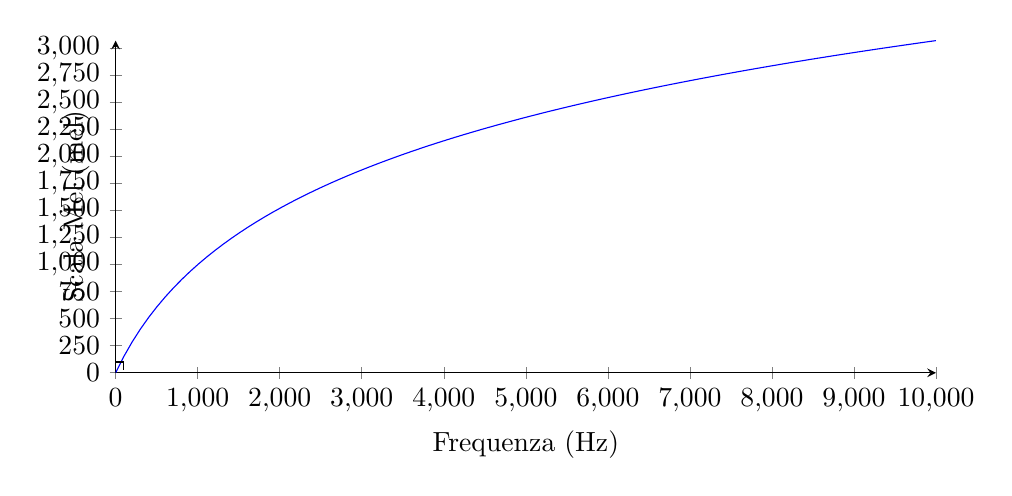
\begin{tikzpicture}
		\begin{axis}[
			width=120mm,
			height=58mm,
			axis lines=left,
			domain=0:10000,
			samples=100,
			no markers,
			xlabel=Frequenza (Hz),
			ylabel=Scala Mel (mel),
			y label style={at={(axis description cs:-0.02,.5)}},
			xtick distance=1000,
			ytick distance=250
			]
			\addplot {2595 * log10(1+x/700)};
			\vertLineFromPoint{100,100};
			\horLineFromPoint{100,100};
		\end{axis}
	\end{tikzpicture}
	\caption{Grafico della scala mel.}
	\label{fig:scala-mel}
\end{figure}